%% LaTeX2e class for student theses
%% sections/content.tex
%% 
%% Karlsruhe Institute of Technology
%% Institute for Program Structures and Data Organization
%% Chair for Software Design and Quality (SDQ)
%%
%% Dr.-Ing. Erik Burger
%% burger@kit.edu
%% burger@kit.edu
%%
%% Version 1.3.3, 2018-04-17


\chapter{Untersuchung von nachrichtenbasierter Middleware}
\label{ch:mom}
Um die Performance einer MOM oder eines Software-Systems im Allgemeinen, vorhersagen zu können, benötigt es zunächst Informationen über die Struktur, sein Verhalten, seiner Ausführungsumgebung und der Benutzung. Dazu müssen die verschiedenen Palladio Rollen relevante Einflüsse bestimmen können. Der Komponenten-Entwickler muss RessourceDemands und Fehlerraten bestimmen. Der Systemdeployer muss verfügbare Rechenleistung und Hardware bestimmen. Der Domänenexperte muss das Verhalten der Nutzer bestimmen. Schließlich muss der Softwarearchitekt fehlende Werte bestimmen und das Modell damit kalibrieren. Diese Modellkalibrierung ist ein wichtiger Bestandteil des Modellierungsprozesses. In \cite{palladio17} wird beschrieben, wie und mit welchen Techniken die verschiedenen Rollen diese Daten erhalten und die jeweiligen Modelle kalibrieren können. Modellkalibrierung ist dabei die Anreicherung von Modellen mit quantitaitven Daten, wie Ressourcenbedarf. Die Daten können aus Messungen oder Vorhersagen stammen. Die Modellkalibrierung ist eine Vorbedingung der Performance-Analyse. Die Informationen die eine Rolle in den verschiedenen Phasen der Software-Entwicklung gewinnen kann sind unterschiedlich. Dieser Prozess lässt sich in drei Phasen strukturieren: Design, Entwicklung und Betrieb. In der Design Phase existiert die Applikation nur auf dem Papier und die Daten, die gesammelt werden können, grobe Schätzungen. Je weiter die Software-Entwicklung fortgeschritten ist, desto mehr quantitative Daten werden verfügbar um die Modelle kalibrieren zu können. Schließlich kann in der Betriebsphase das Gesamtsystem und auch der Benutzer quantitative Daten liefern. 

Im Rahmen der Masterarbeit soll eine MOM modelliert werden um in Performanzanalysen verwendet werden zu können. Dazu müssen, wie oben beschrieben, verschiedenen quantitative Daten gesammelt werden um das Modell kalibrieren zu können um eine Performanzanalyse zu ermöglichen. Dazu soll zunächst eine bereits existierende MOM ausgewählt werden. Da es sich dabei um eine bereits existierende MOM handelt, befindet sie sich im letzten Schritt der drei Software-Entwicklungsphasen. Somit lässt sich das Gesamtsystem betrachten und ausmessen um quantitative Daten zu sammeln. Zunächst werden in \autoref{sec:anforderungenMom} Anforderungen an die MOM Auswahl definiert um dann im nächsten Schritt die ausgewählte MOM in \autoref{sec:rmq} vorzustellen. Schließlich soll diese mit einem Werkzeug ausgemessen werden. Die Ergebnisse werden in \autoref{sec:rmqBenchmark} vorgestellt. Diese werden verwendet um die Modelle in \autoref{ch:modellierung} kalibrieren zu können.


\section{Anforderungen an MOMs}
\label{sec:anforderungenMom}
Da es eine Vielzahl von MOMs gibt, muss zunächst eine Auswahl stattfinden. Dazu werden im ersten Schritt der Masterarbeit Anforderungen erarbeitet, die ein MOM erfüllen muss, damit sie in Betracht kommt. Im Rahmen des Proposals wurde sich bereits mit der Frage auseinander gesetzt und die folgenden Anforderungen erarbeitet:
\begin{itemize}
\item Die MOM sollte \textbf{Open Source} sein.
\item Sie sollte eine \textbf{weite Verbreitung} haben. Um dies einzuschätzen zu können sollen verschiedene Entwicklerforen wie Stackoverflow und Stachshare untersucht werden, sowie die Literatur in diesem Bereich.
\item %Da sowohl das Experimentsystem eine Java und das Evaluierungssystem eine C++ Implementierung besitzen sollte 
Die MOM sollte \textbf{Programmiersprachen unabhängig} sein.
\item Sich in \textbf{aktiver Entwicklung} befinden.
\item Bereits gesammelte \textbf{Erfahrung} mit MOMs.
\end{itemize}
%- bestimmte Protokolle unterstuetzen \\ %(https://www.predic8.de/activemq-hornetq-rabbitmq-apollo-qpid-vergleich.htm)

%\section{Auswahl der MOMs}
%In diesem Schritt sollen zwei bis drei MOMs ausgewählt werden. Dabei sollen die zuvor erarbeiteten Anforderungen einbezogen werden. Da sich bereits im Rahmen des Proposals mit dem Thema auseinander gesetzt wurde, wurden bereits drei starke Kandidaten identifiziert, die die bereits erarbeiteten Anforderungen erfüllen.
Im Folgenden soll ein System untersucht werden, das diese Anforderungen erfüllt.

\section{RabbitMQ}
\label{sec:rmq}
RabbitMQ ist, mit 35,000 aktiven Produktivumgebungen, eine der am weitesten verbreitete MOM. 
RabbitMQ ist eine Open-Source-MOM, die seit 2007 entwickelt wird \cite{rabbitmq}. Das Ziel von RabbitMQ ist es allgemein einsetzbar zu sein. Deshalb wird eine Vielzahl an Protokollen unterstützt, unter anderem das JMS Protokoll. RabbitMQ kann auf einem zentralen Konten oder auf mehreren verteilten Knoten eingesetzt werden. Für den Nachrichtenaustausch verwendet RabbitMQ Warteschlangen. Diese lassen sich unterschiedlich konfigurieren, zum Beispiel die Warteschlangenlänge. Das kommunizieren zwischen Sender und Empfänger geschiet dabei nicht direkt über die Warteschlange. Nachrichten werden zunächst an einen Exchange gesendet. Dieser ist für das richtige weiterleiten an die passende Warteschlange verantwortlich. Dies geschieht mit Hilfe von Bindungen und Routing-Schlüßeln. In RMQ ist eine Bindung ist eine Verbindung zwischen einer Warteschlange und einem Exchange. RabbitMQ unterscheidet zwischen vier verschiedenen Exchanges:
\begin{itemize}
    \item Direkt: Hierbei meldet sich eine Warteschlange mit einem bestimmten Routing-Schlüssel (RK) X beim Exchange an. Wenn eine Nachricht mit einem RK Y ankommt, wird sie nur an die Warteschlange gesendet, wenn die RKs X und Y übereinstimmen.
    \item Topik: Die Warteschlange ist mit einem Binding an den Exchange gebunden. Nachrichten werden wieder anhand des RK weitergeleitet. Der RK muss nicht mehr genau passen, sondern muss auf ein bestimmtes Muster aufweisen.
    \item Fanout: Die ankommende Nachricht wird an alle am Exchange angemeldeten Warteschlangen gesendet. Der RK wird dabei ignoriert.
    \item Header: Dabei werden die Attribute des Nachrichtenkopfes verwendet, um die Nachricht weiterzuleiten.
\end{itemize}
Diese Architektur erlaubt verschiedene Interaktionstypen. Sowohl eins-zu-eins als auch viele-zu-viele Interaktionen sind möglich. Dabei können nicht nur mehrere Warteschlangen existieren, sondern auch mehrere Exchange und jede Komponente auf einem anderen Knoten verteilt. Aufgrund dieser Architektur hat RMQ auch einen hohen Grad der Entkopplung. Den Sender und Empfänger müssen sich nicht kennen, sie kommunizieren lediglich über den Exchange miteinander (Raum). Weder der Sender noch der Empfänger müssen zur gleichen Zeit aktiv sein. Der Sender sendet Nachrichten an die Warteschlange und der Empfänger holt sie raus, wenn er dazu die Ressourcen hat (Zeit). Schließlich müssen Sender und Empfänger nicht aufeinander warten, da sie über eine Warteschlange kommunizieren (Synchronisation).
In \autoref{img:rmq_architecture} ist ein Beispiel für eine mögliche RMQ-Architektur und Kommunikation zwischen Sendern und Empfängern dargestellt. Dabei ist ExhangeA vom Typ Direkt. Dieser ist mit WarteschlangeA verbunden. ExchangeB ist ein Topic-Exchange und mit WarteschlangeB und WarteschlangeC verbunden. Dabei unterscheiden sich die beinden Bindungen in ihrem Routing-Muster. EmpfängerA empfängt Nachrichten aus WarteschlagenA und EmpfängerB Nachrichten aus WarteschlangeB und WarteschlangeC. Wenn ein Sender eine Nachricht an ExchangeA sendet, wird diese in WarteschlangeA abgelegt, wenn der Routing-Schlüssel der Nachricht mit dem Routing-Schlüßel der Warteschlange übereinstimmt, da diese über eine direkte Bindung mit dem Exchange verbunden ist. Wenn eine Nachricht an ExchangeB gesendet wird, wird anhand des Routing-Musters entschieden, ob die Nachricht an WarteschlangeB oder WarteschlangeC gesendet wird. 
\begin{figure}
\center
  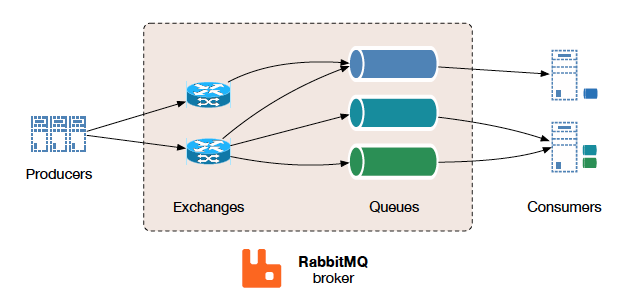
\includegraphics[width=1\textwidth]{images/measurement/rmqexample.png}
  \caption{beispiel einer Kommunikation in RMQ}
  \label{img:rmq_architecture}
\end{figure}
%https://www.cloudamqp.com/blog/2015-05-18-part1-rabbitmq-for-beginners-what-is-rabbitmq.html

%https://www.cloudamqp.com/blog/2018-01-08-part2-rabbitmq-best-practice-for-high-performance.html
Da in dieser Arbeit der Fokus auf der Performance einer MOM liegt, wurden in Literatur Möglichkeiten untersucht, mit denen eine hohe Performance in RMQ erreicht werden kann. Dazu konnten in (Rmqbuchh) die folgenden Vorgehensweise identifiziert werden. RMQ funktioniert am besten, wenn der Füllstand einer Warteschlange klein gehalten wird. Ein Nachricht die in eine leere Warteschlange abgelegt wird, geht direkt an einen Empfänger. Je mehr Nachrichten sich in der Warteschlange befinden, desto länger dauert es diese zu bearbeiten. Wenn der Durchsatz eine wichtige Rolle spielt und die Warteschlangen nicht voll laufen sollen, ist das setzen einer maximal Länge der Warteschlange oder das setzen einer Lebensdauer für Nachrichten empfohlen. Dabei bleibt die Warteschlange kurz und neue Nachrichten werden vom Kopf der Warteschlange verworfen, falls sie länger als festgelegt wird. Ein weiterer Performance-Einfluss haben Lazy-Warteschlangen. Dabei werden die Nachrichten einer Warteschlange direkt auf die Festplatte, anstatt in den Hauptspeicher, geschrieben. Das Ziel dabei ist, sehr lange Warteschlange unterstützen zu können. Dies kann aus verschiedenen Gründen nötig sein. 
\begin{itemize}
    \item Empfänger können aus verschiedenen Gründen ausfallen
    \item Plötzlicher anstieg ankommender Nachrichten
    \item Empfänger sind langsamer als normal
\end{itemize}
Das heißt die Hauptziele dieser Konfiguration sind vor allem Zuverlässigkeit. Im Fall das Performance bevorzugt wird, sollte also auf Lazy-Warteschlangen verzichtet werden. Schließlich kann der Durchsatz dadurch erhöht werden, wenn mehrere Warteschlangen verwendet werden. Zum Einen kann eine einzelne Warteschlange nicht mehr als ca. 50.000 Nachrichten bearbeiten. Zum anderen sind Warteschlangen einfädig. Das heißt, dass der beste Durchsatz auf einem System möglich ist, bei dem es genau so viele Warteschlangen wie Kerne hat. 

In der Folgenden Ausmessung von RMQ wurden diese und weitere Konfiguration untersucht um zu prüfen ob sie einen messbaren Einfluss auf die Performance haben.

\section{Benchmark}
Im Folgenden soll RMQ ausgemessen werden um quantitative Daten ableiten zu können. Dazu wird in \autoref{sec:testmachine} zunächst die Testmanschinen vorgestellt, mit denen die Messungen durchgeführt wurden. Im Anschluss werden in \autoref{sec:rmqBenchmark} die Ergebnisse der einzelnen Messungen vorgestellt und in \autoref{sec:rmqZusammenfassung} zusammengefasst.

\subsection{Testmaschinen}
\label{sec:testmachine}
In diesem Abschnitt sollen die benutzten Maschinen Dokumentiert werden, mit denen RMQ ausgemessen wurde. Für die Messungen wurden zwei Testmaschinen benutzt. Die Systemspezifikation sind in \autoref{tab:systespec} aufgelistet. Beide Systeme haben die gleiche Systemspezifikation und haben RMQ Version 3.7.8 installiert. Im Folgenden werden die beiden Systeme verwendet um RMQ auszumesse.

\begin{table}
  \begin{tabular}{|l|l|l|l|l|l|}
    RAM & Speicher & VCPUs & GHZ & Netzwerk & OS \\
    \hline
     4 & 15 & 2 & 2.4 GHZ & Netzwerk & Ubuntu 18.04
  \end{tabular}
	\caption{\label{tab:systespec} BWCloud VMs}
\end{table}

\subsection{Ausmessung von RMQ}
\label{sec:rmqBenchmark}
Im Folgenden soll RMQ ausgemessen werden um mit den Ergebnissen die Modelle kalibrieren zu können. Um RMQ auszumessen wurde das Performance-Werkzeug von RMQ benutzt. Dieses erlaubt es die gesendeten und empfangenen Nachrichten und ihre Latenz zu messen. Dabei ist die Zeit gemeint, die eine Nachricht braucht bis sie vom Empfänger aus der Warteschlange herausgenommen wird, nachdem sie vom Sender dort abgelegt wurde. Das Werkzeug kann konfiguriert werden um bestimmte Szenarien zu simulieren. Unter anderem lässt sich die Anzahl der zu sendenden und zu empfangenen Nachrichten pro Sekunde einstellen. Eine weitere Konfiguration ist das einstellen bestimmte Nachrichtengrößen. Im Folgenden sollen die Ergebnisse der Messungen vorgestellt werden. Dabei werden die einzelnen Ergebnisse und ihr Versuchsaufbau vorgestellt. Jedes Ergebnis wird wie folgt beschrieben: 
\begin{itemize}
    \item Vorstellung des Szenarios
    \item Beobachtungen des Systemverhaltens
    \item Messergebnisse
\end{itemize}
Jede Messung wurde zehn mal durchgeführt. Die einzelnen Konfiguration wurde jeweils zwei Minuten ausgeführt. 



\subsubsection{Latenz einer Nachricht}
\label{sec:oneMsgLatency}
Zunaechst soll geprueft werden wie die Latenz einer einzelnen Nachricht ist. Dabei wurde auch die groesse einer Nachricht betrachtet. Dazu wurde die Senderate auf eine Nachricht pro Sekunde reduziert und die Nachrichtengroesse varriert zwischen 100 Byte und 100.000 Bytes.
%B
Die Ergebnisse sind in \autoref{img:senderate1-A} zu sehen. Dabei ist zu sehen, dass die Latenz mit Ansteigen der Groesse auch waechst. 
%Im durchshnitt kann man eine Latenz von 2627 Mikrosekunden beobachten. In \autoref{img:senderate1-B} sind die Ergebnisse mit Testsystem B zu sehen. Hier wird im durchshnitt eine hoehere Latenz von 29237 Mikrosekunden beobachten. 
\begin{figure}
\center
  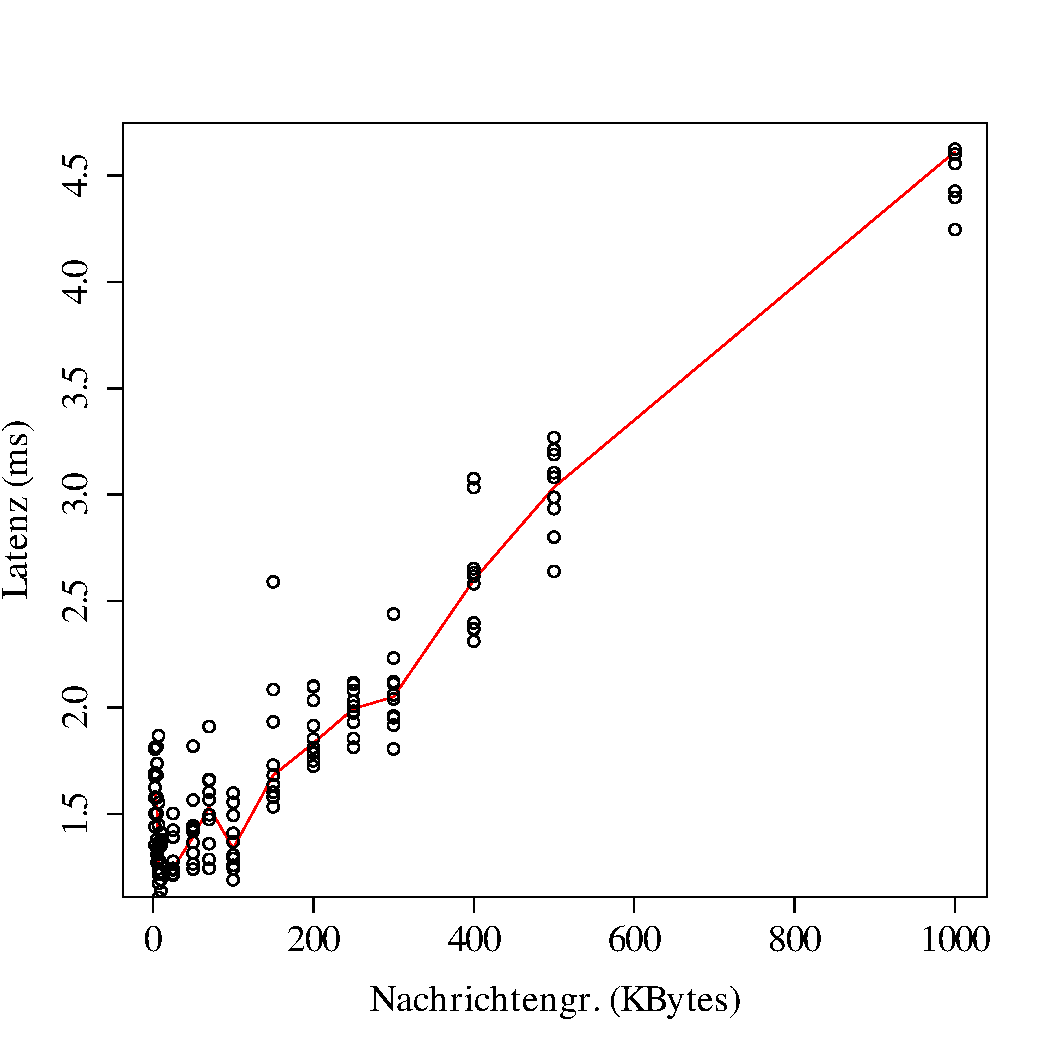
\includegraphics[width=0.5\textwidth]{images/measurement/rate-limit-1-A.pdf}
  \caption{Senderate 1/sec, Testsystem A}
  \label{img:senderate1-A}
\end{figure}
Als naechstes wurde die Latenz zu einem entfernten RMQ Broker gemessen. Das System auf dem der entfernte Broker laeuft hat die selben spezifikationen wie das in \autoref{sec:testmachine} beschriebene. Die ausgemssenene Netzwerklatenz betrug 1ms. Die Senderate und Nachrichtengroesse sind wie oben beschrieben. Die Ergebnisse sind in \autoref{img:senderate1-B} zu sehen. Auch hier waechst die Latenz mit Ansteigen der Groesse. Im Unterschied zu ersten Messung ist die Latenz einer Nachricht groesser. 
%E
Die laengere Latenz in der zweiten Messung laesst sich auf die Netzwerklatenz zurueckfuehren. Somit ist neben der Nachrichtengroesse auch die Netzwerklatenz ein Faktor, der die Latenz einer Nachricht beeinflusst.

\begin{figure}
\center
  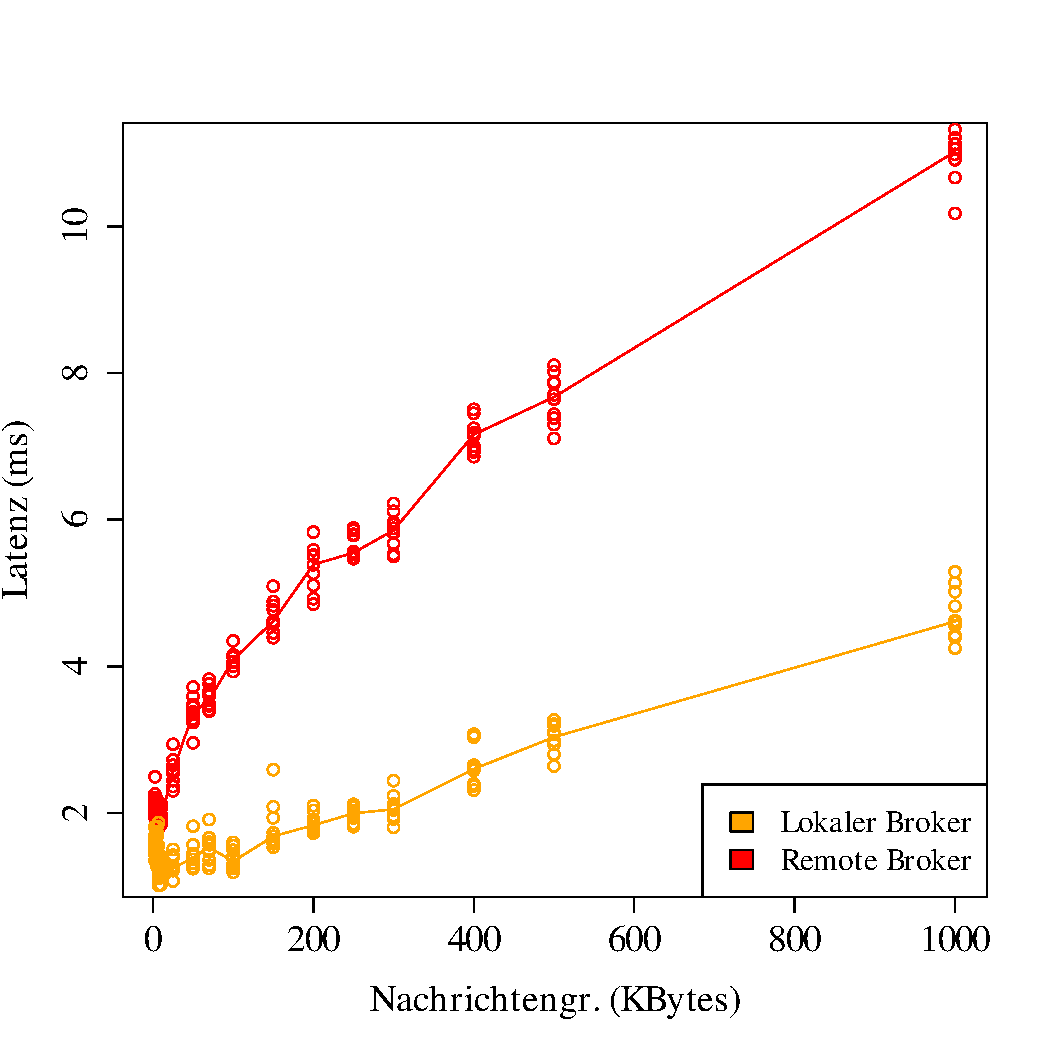
\includegraphics[width=0.5\textwidth]{images/measurement/rate-limit-1-AvsB.pdf}
  \caption{Senderate 1/sec, Testsystem A}
  \label{img:senderate1-B}
\end{figure}

\subsubsection{Nachrichtengroesse}
Im Folgenden sollen weitere Effekte im zusammenhang mit der Nachrichtengroesse untersuch werden. Dazu wurde die Limitierung der Senderate aufgehoben. Die Nachrichtengroessen variieren zwischen 100 Byte bis 1.000.000 Bytes.
%B
In \autoref{img:msgsize} sind die Auswirkung der Nachrichtengroesse auf die Senderate und die insgesamt gesendete Datenmenge zu sehen. dabei ist zu sehen, dass mit zunehmender groesse die Nachrichtenmenge die pro Sekunde gesendet werden kann, abnimmt. Gleichzeitig nimmt aber die insgesammt gesendete Datenmenge, in Bytes, zu. 
\begin{figure}
\center
  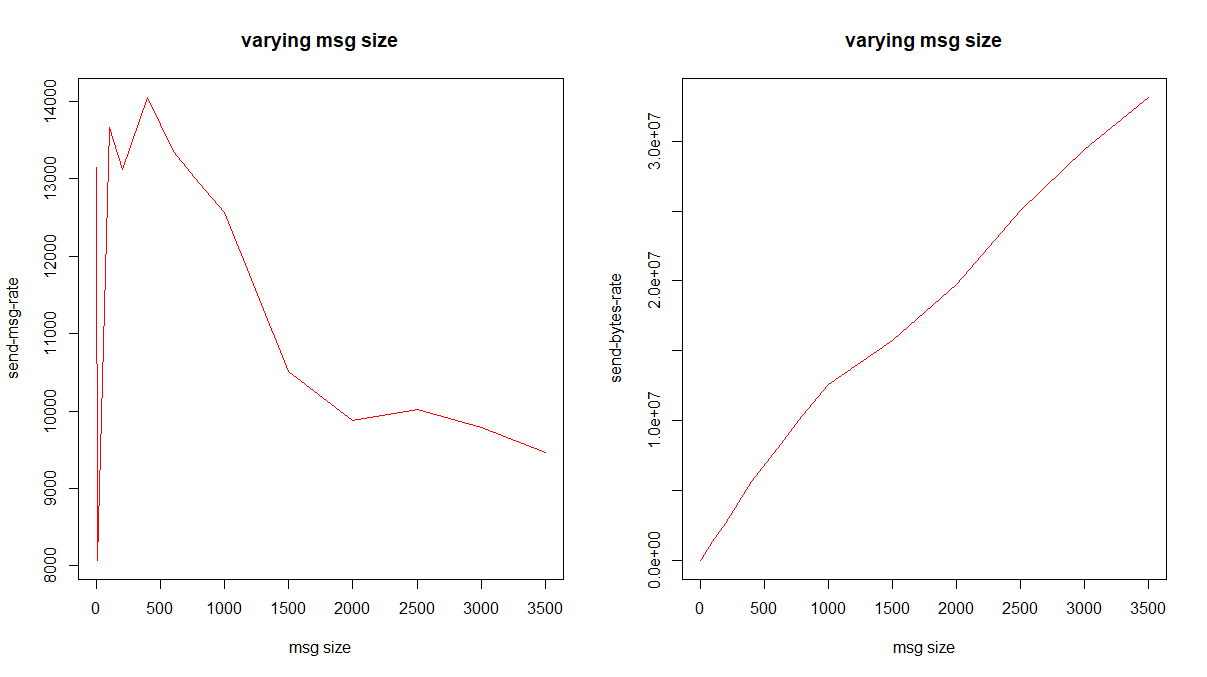
\includegraphics[width=1\textwidth]{images/msg-size.png}
  \caption{Senderate 1/sec, Testsystem B}
  \label{img:msgsize}
\end{figure}
%E
Dieser Effekt laesst sich darauf zurueckfuehren, dass bei groesseren Nachrichten der Broker weniger routing overhead hat.
%https://www.rabbitmq.com/blog/2012/04/25/rabbitmq-performance-measurements-part-2/

\subsubsection{Maximale zu sendende Datenmenge}
\label{sec:maxthroughput}
Nachdem die Effekte der zueahmende Nachrichtengroesse grprueft wurden, soll nun geprueft werden wie gross die insgesammt moegliche Datenmenge die gesendet und empfangen werden kann ist. Dazu wurden Nachrichten unterschiedlicher Groesse gesendet. Die Nachrichten waren zwischen 100 Bytes und 200000 Bytes (2MB) gross. Es wurden zwei Messungen durchgefuehrt. Die erste war mit einem Sender und keinem Empfaenger. Die zweite mit einem Sender und einem Empfaenger. 
%B
Die Ergebnisse sind in \autoref{img:maxByteThroughputA} zu sehen. Die Abbildung zeigt, dass wenn kein Empfaenger vorhanden ist, mit zunehmender Nachrichtengroesse die insgesamt gesendete Datenmenge an einen Wert bei ca. 230 MByte/s annaehert. Wenn ein Empfaenger vorhanden ist, naehert sich die Datenmenge an 174 MByte/s an.
\begin{figure}
\center
  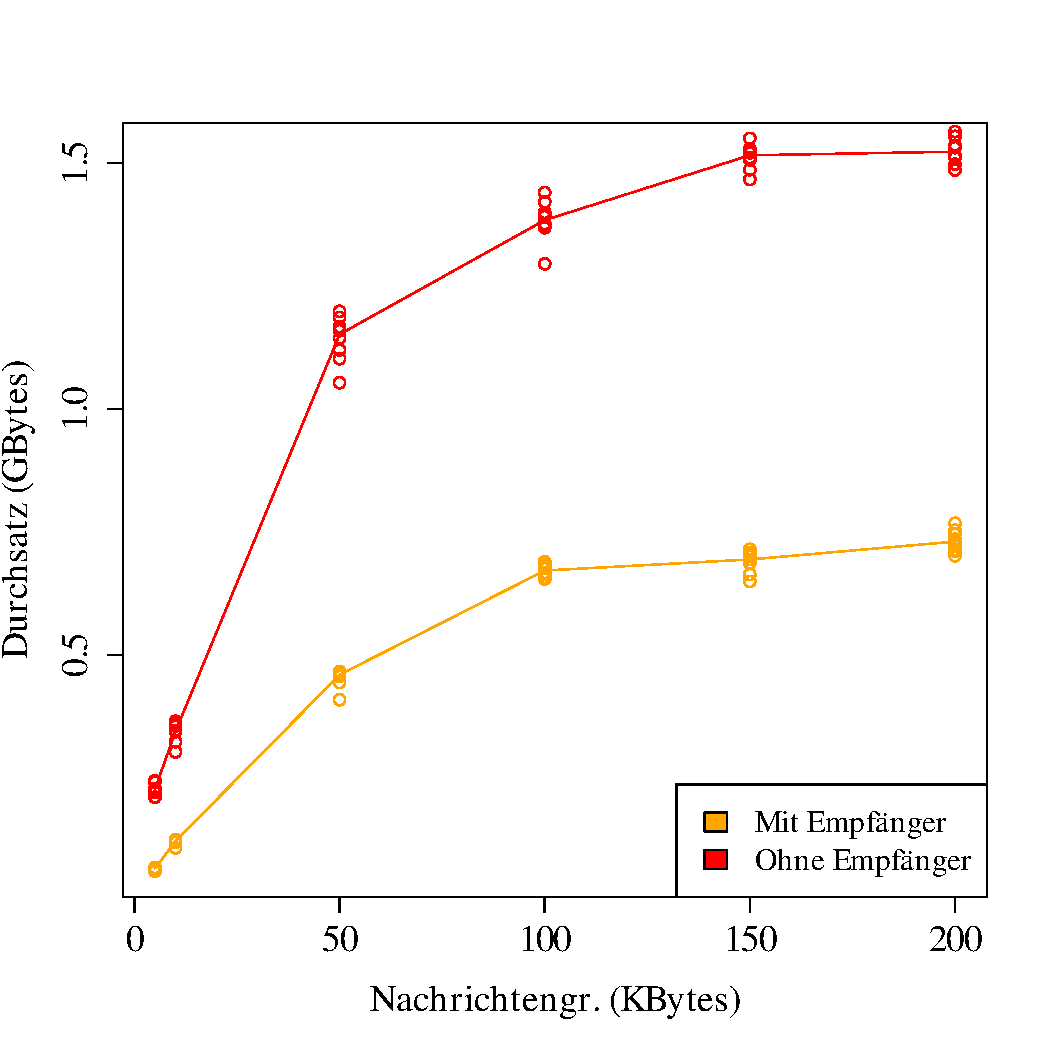
\includegraphics[width=1\textwidth]{images/measurement/rate-limit-unlimited-consumer-vs-no-consumer.pdf}
  \caption{Max Datenmenge ca. 230/174 (kein Empfaenger/mit Empfaenger), Testsystem A}
  \label{img:maxByteThroughputA}
\end{figure}

Ein weiterer Effekt ist in \autoref{img:unlimitedLatency} zu sehen. Dabei ist zu sehen, dass die Latenz sinkt wenn mehr Nachrichten auf einmal gesendet werden.
\begin{figure}
\center
  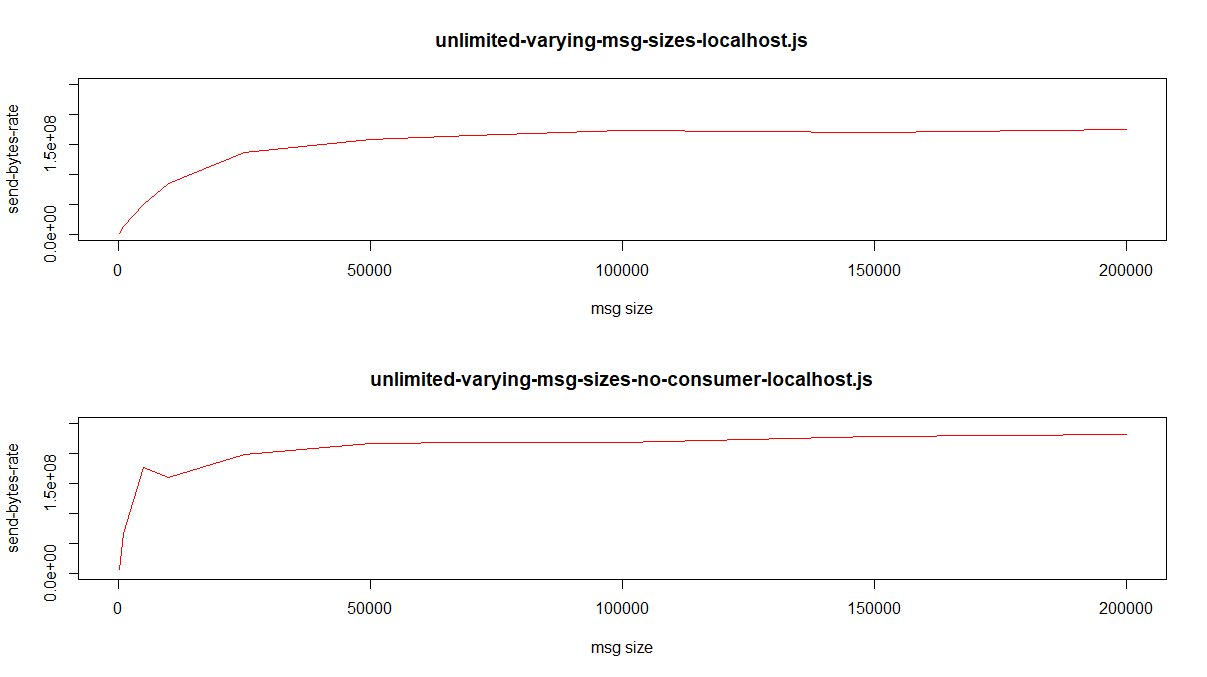
\includegraphics[width=1\textwidth]{images/max-byte-throughput-A.pdf}
  \caption{Max Datenmenge, Latenz, Testsystem A}
  \label{img:unlimitedLatency}
\end{figure}
Dieser Effekt laesst sich darauf zurueckfuehren, dass wenn mehrere Nachrichten auf einmal gesendet werden der Broker weniger routing overhead hat.

Die selbe Messung wurde an dem enfernten Testsystem B ausgefuehrt. Die gegenueberstellung fuer den Fall ohne Empfaenger ist in \autoref{img:maxByteThroughputNoConsumerB} zu sehen. Die an das System B gesendete Datenmenge ist um den Faktor (ca 3) kleiner. Die Messung mit Empfaenger ist in \autoref{img:maxByteThroughputB} abgebildet. In diesem Fall ist die an das System B gesendete Datenmenge um den Faktor (ca 2) kleiner.
\begin{figure}
\center
 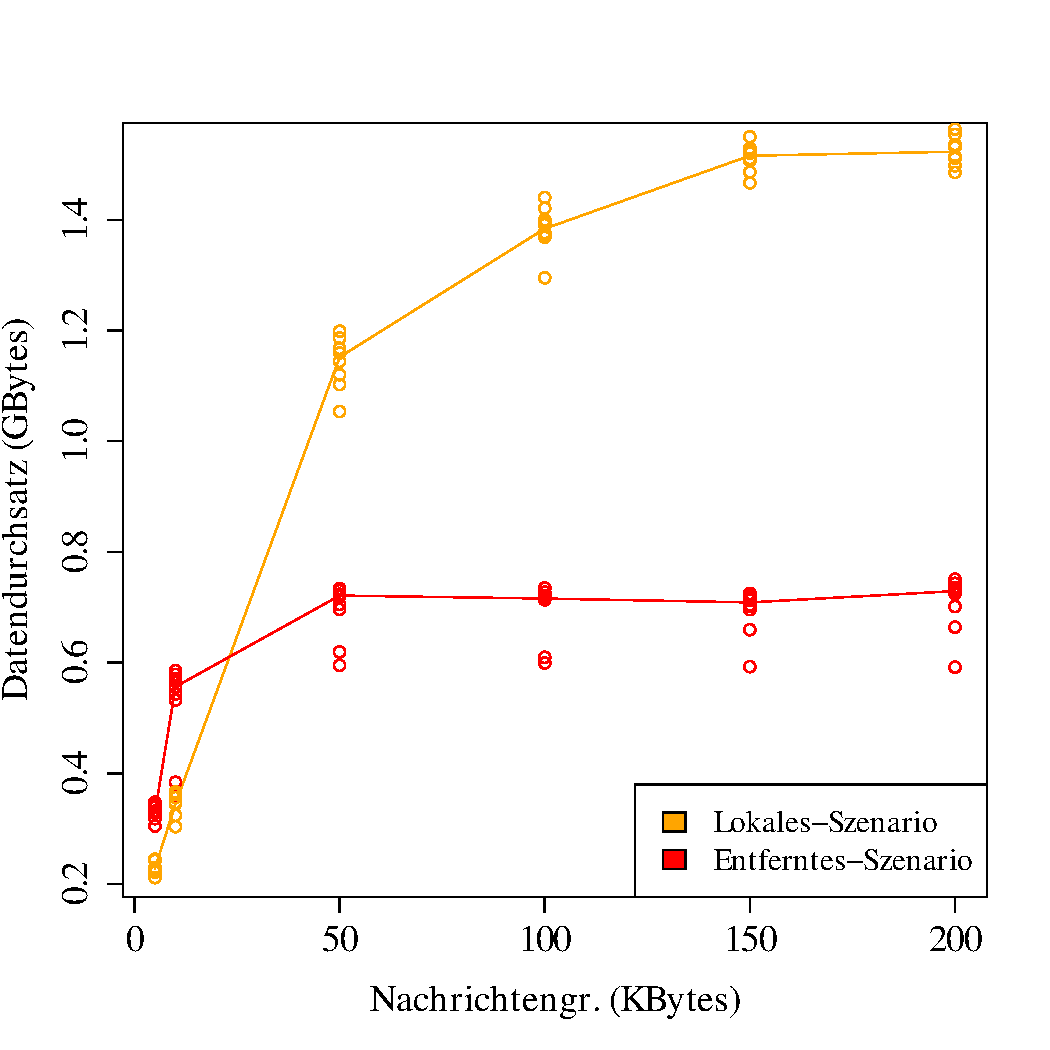
\includegraphics[width=1\textwidth]{images/measurement/rate-limit-unlimited-no-consumer-AvsB.pdf}
  \caption{Max Datenmenge ohne Empfaenger (Remote)}
  \label{img:maxByteThroughputNoConsumerB}
\end{figure}
\begin{figure}
\center
 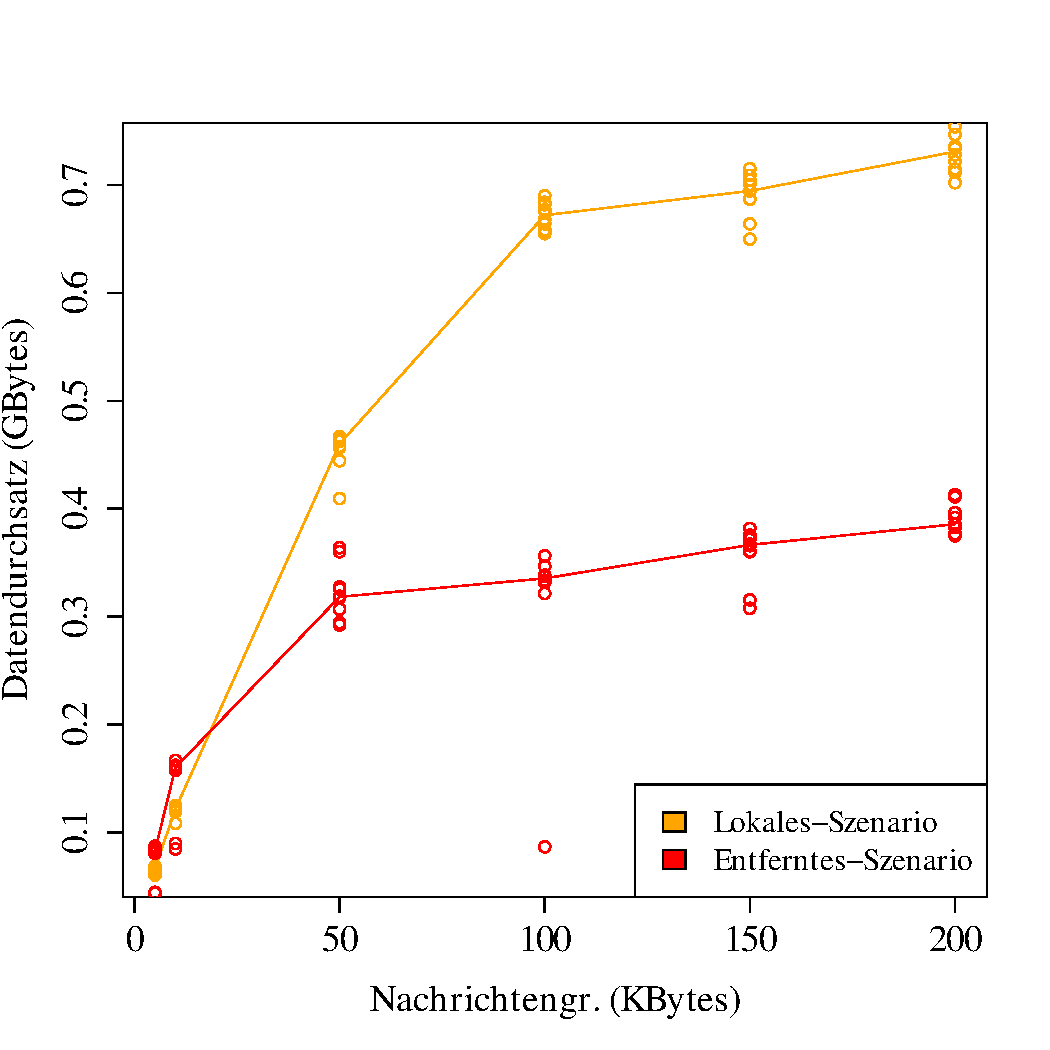
\includegraphics[width=1\textwidth]{images/measurement/rate-limit-unlimited-AvsB.pdf}
  \caption{Max Datenmenge mit Empfaenger (Remote)}
  \label{img:maxByteThroughputB}
\end{figure}
%E
Obwohl beide Testmaschinen vom selben Anbieter sind, unterscheiden sich die moeglichen Datenmengen zwischen einem lokalen und entfernten Broker. Diesen unterschied kann auf den moeglichen Durchsatz einer Netzwerkverbingung zuruckgefuehrt werden. Somit ist der moegliche Durchsatz einer Verbindung zwischen Sender, Empfaenger und dem Broker ein limitierender Faktor und hat somit auch einfluss auf die Performanz des Gesamtsystems.


\subsubsection{MaxLength}
\label{subsub:maxlength}
RMQ erlaubt es die Warteschlangen groesse zu limitieren. Ausserdem kann eine Strategie festgelegt werden, was mit ankommenden Nachrichten passieren soll. Im Standardfall wird der Kopf der Warteschlange verworfen. Dies sollte mit der folgenden Messung untersucht werden. Dazu wurde mehrere Warteschlange angelegt. Diese hatten eine Maximallaenge von 100, 5000 und 50.000. Die Groesse von 50.000 ist die RMQ standard groesse fuer Warteschlangen. Damit man die Auswirkung auf volle Warteschlangen sehen kann wurde die Sende- und Empfangsrate entsprechend angepasst. Die Senderate wurde auf 1000 und die Empfangsrate auf 100 Nachrichten die Sekunde eingestellt. Die Nachrichten groesse betraegt 100 Bytes.
%B
Die Ergebnisse sind in \autoref{img:maxlength} zu sehen. Zu sehen ist, dass die Latenz bei den begrenzten Warteschlangen ab einem bestimmte Zeitpunkt nicht weiter anwaechst. Die Latenz der unbegrenzten Warteschlange waechst dagegen immer weiter.
\begin{figure}
\center
  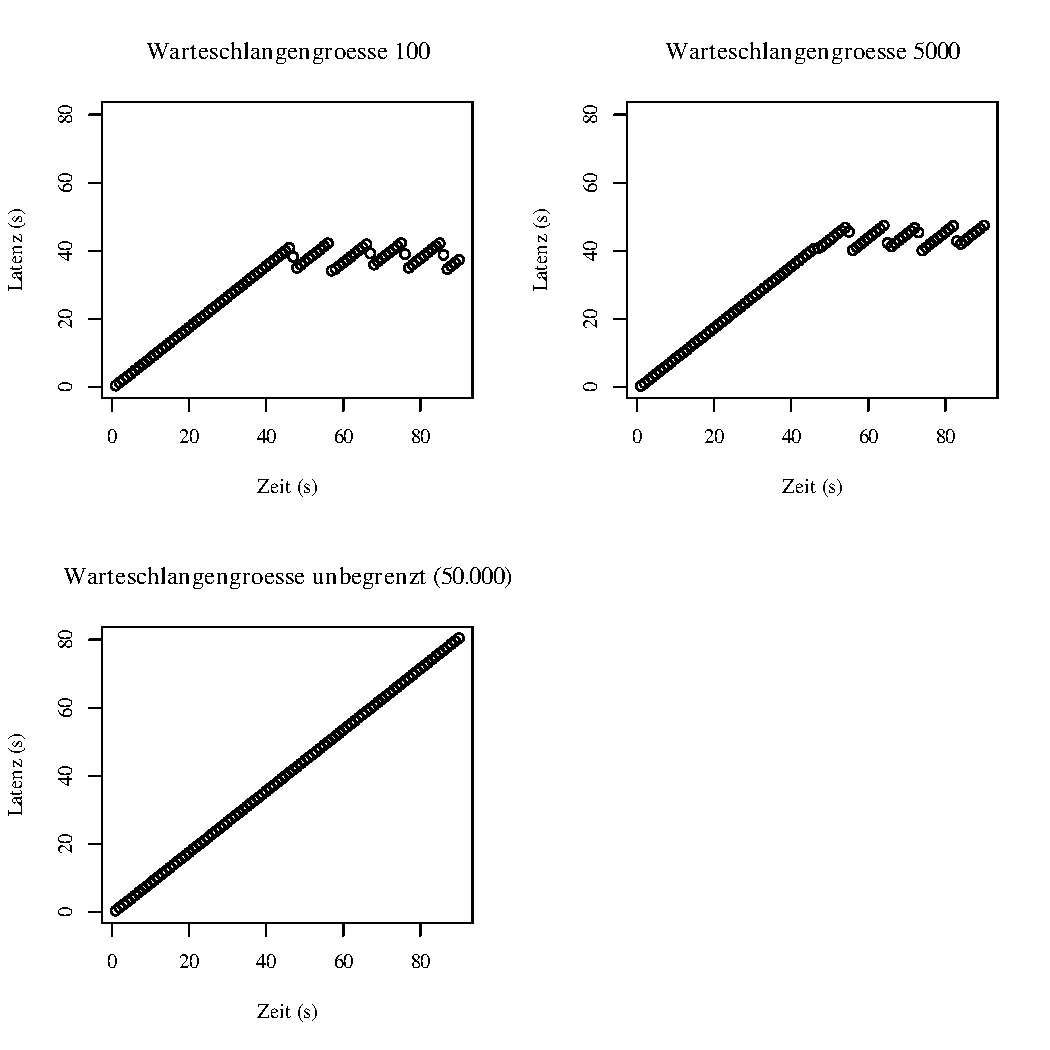
\includegraphics[width=1\textwidth]{images/measurement/max-length.pdf}
  \caption{Senderate 1000/sec, Empfangsrate 100/sec}
  \label{img:maxlength}
\end{figure}
%E
Diese Konfiguration zeigt, dass die Warteschlangenbegrenzung einen Einfluss auf die Latenz hat und man diese gering halten kann, wenn man die Warteschlangengroesse begrenzt. Der Nachteil dabei ist, dass Nachrichten verworfen werden, sobald die Warteschlange voll ist. Somit hat auch die Warteschlangengroesse einen Einfluss auf die Performanz. 

%wenn Queue voll, dann wird Msgrate angepasst

%Flow alarm ab RabbitMQ 2.8.0+ bei Versionen davor verhlaehlt sich RMQ wie in (sec: Speicher ausgeschoepft)

\subsubsection{Speicher von RMQ ausgeschoepft}
Nachdem in der Messung davor die Laenge der Warteschlange betrachtet wurde, soll nun untersucht werden ob der Verfuegbare Speicher des Broker einfluss auf die Performanz hat. Dazu wurde auf der Testmaschine B die Hauptspeicher fuer RMQ auf 10 MB gesetzt.  
Sollte der verfuegbare Speicher des Broker ausgeschoepft sein, wird der MemoryAlarm aktiviert und der Broker blockiert ankommende Nachrichten, bis der Speicher wieder frei ist. Dies ist in (abb) zu sehen.
TODO beobachtung und Ergebnis

\subsubsection{Ansteigen der Queuelaenge}
\label{sec:queueGrowth}
TODO: \\
Sender 2 Nachrichten \\
Empfaenger 1 Nachricht \\
evtl. mehrere Verhaeltnisse \\
Fuellstand der Queue steigt an \\

\subsubsection{Lazy Queues}
\label{sec:rmqLazy}
In der naechsten Messung soll untersucht werden ob die Konfiguration von Lazy-Warteschlangen Auswirkungen auf die Performance hat. Die Senderate wurde auf eine Nachricht pro Sekunde limitiert. Die groesse der gesendeten Nachrichten varriieren zwischen 100 Byte und 100.000 Bytes.
%B
In \autoref{img:lazy} ist ein Vergleich der Messung aus \autoref{sec:rate1} und den Messergebnissen mit Lazy Warteschlangen abgebildet. Zu sehen ist, dass die Latenz mit Lazy Warteschlangen groesser ist, als ohne.
\begin{figure}
\center
  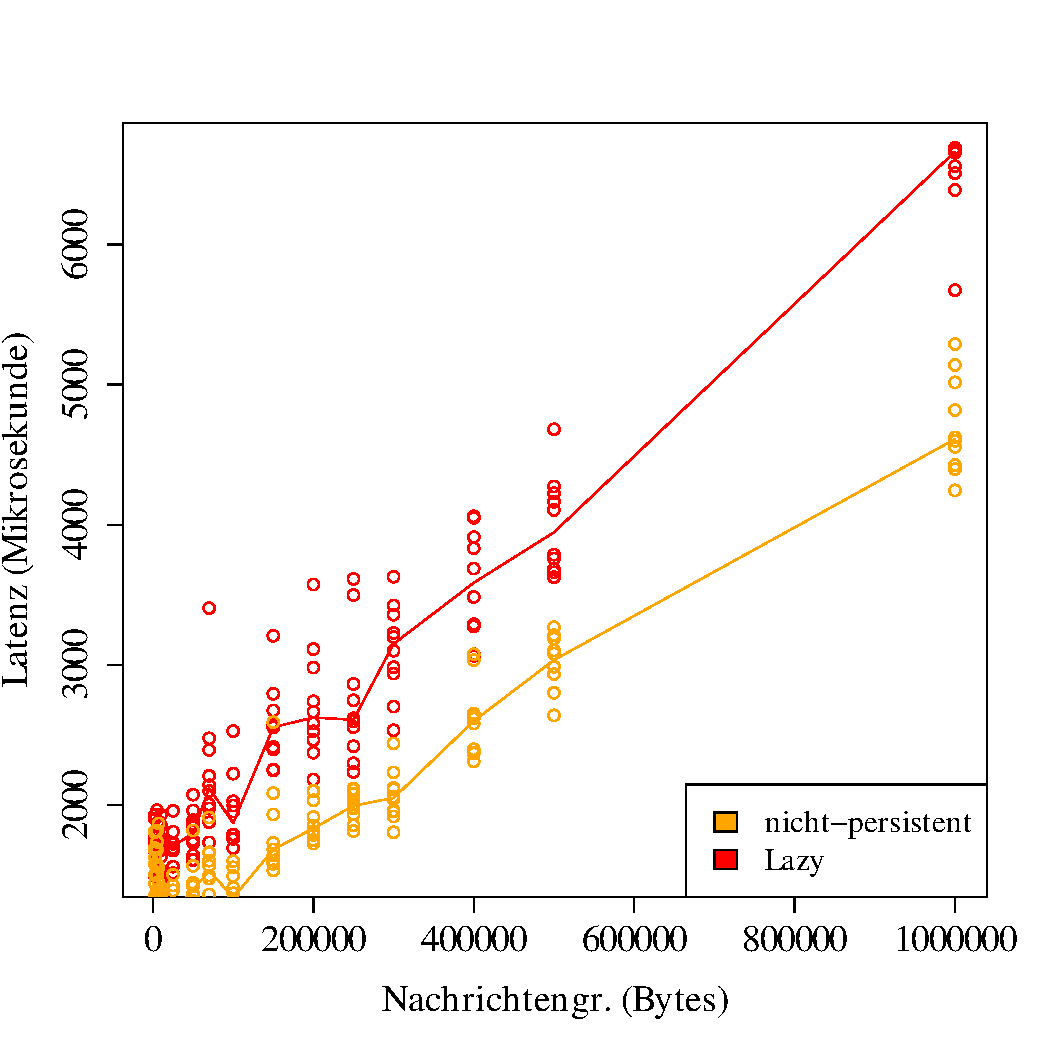
\includegraphics[width=1\textwidth]{images/measurement/lazy-queues.pdf}
  \caption{Lazy Queue vs not Lazy Queue}
  \label{img:lazy}
\end{figure}
%E
Grund hierfuer ist das die Nachrichten auf die Festplatte anstatt in den Hauptspeicher geschrieben werden. Somit hat der Ort an den Nachrichten gespeichert werden einen Einfluss auf die Performanz.



\subsubsection{Mehrere Empfaenger}
In \autoref{subsub:maxlength} war bereits zu sehen, dass volle Warteschlangen einen Einfluss auf die Latenz haben. In dieser Messung soll geprueft werden ob mehrere Empfaenger eine Warteschlange genauso schnell abarbeiten koennnen wie ein einzelner und somit die Latenz gemeinsam in den Griff bekommen koennen. Dazu wurde die Senderate eines Senders auf 1000 Nachrichten und die Empfangsrate auf 200 Nachrichten pro Sekunde limitiert. Alle Empfaenger greifen auf die selbe Warteschlange zu. Ausserdem wurde eine Referenzmessung mit einem Sender und einem Empfaenger mit einer Empfangsrate von 1000 durchgefuehrt.
%B
In \autoref{img:varyingConsumer} sind die Ergebnisse der Messung zu sehen. Darin ist zu sehen, dass ein Empfanger mit gedrosselter Empfangsrate nicht hinterherkommt die Warteschlange abzuarbeiten und somit die Latenz sehr schnell steigt. Bei zwei Empfaenger, mit einer gemeinsamen Empfangsrate von 400 Nachrichten die Sekunde, steigt die Latenz nicht ganz so schnell, aber auch hier kommen die Empfanger nicht hinterher die Warteschlange abzuarbeiten. Mit fuenf Empfaenger und einer gemeinsamen Empfangsraten von 1000 Nachrichten, schaffen sie es die Warteschlange abzuarbeiten. Im Vergleich zu der Referenzmessung mit einem Empfaenger, beinhaltet die Messung mit mehreren Empfaengern einige Schwankungen.
\begin{figure}
\center
  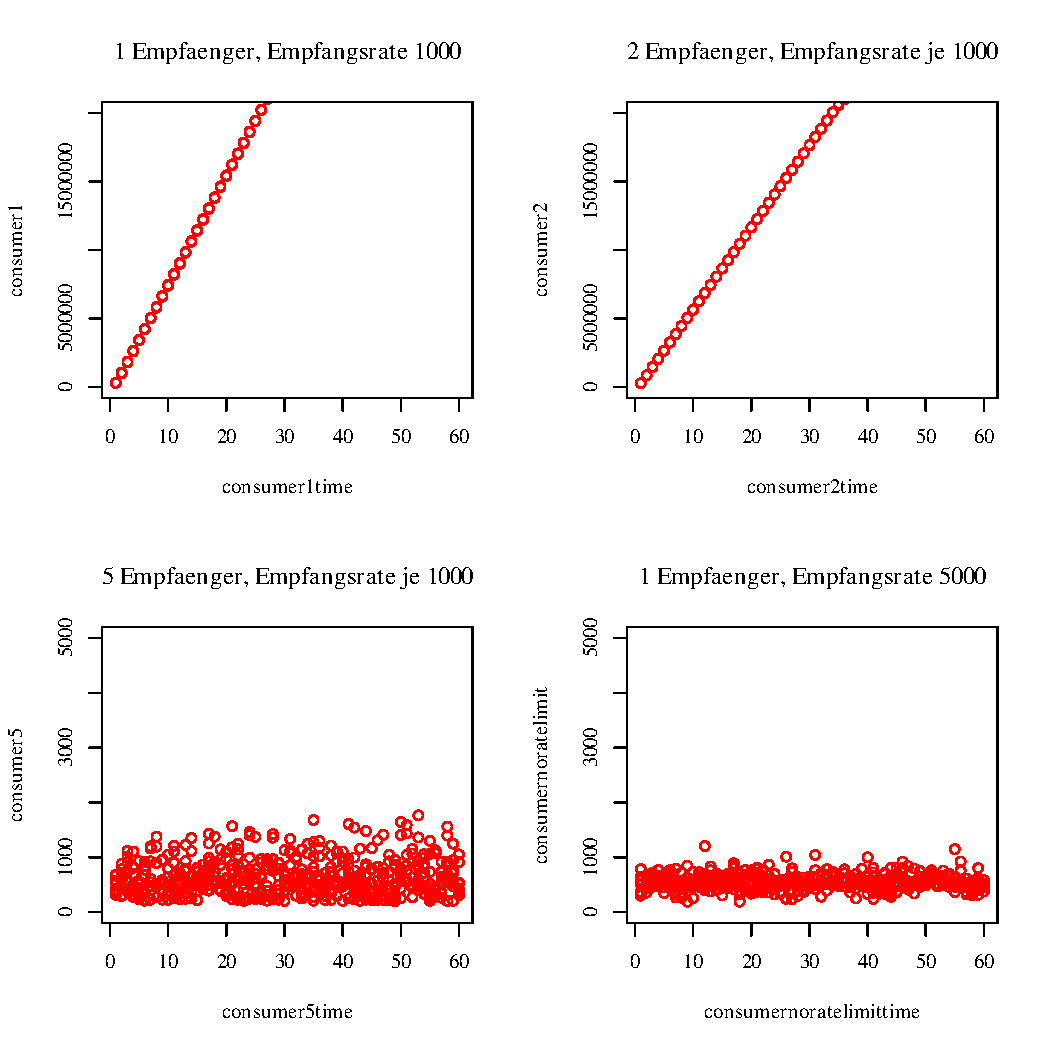
\includegraphics[width=1\textwidth]{images/measurement/varying-consumer.pdf}
  \caption{Verschiedene Empfaenger Anzahl}
  \label{img:varyingConsumer}
\end{figure}
%E
Diese Messung zeigt, dass mehrer Empfaenger eine Warteschlange genauso schnell abarbeiten koennen wie ein einzelner. Die Schwankungen lassen sich mit der synchronisation der Empfaenger erklaeren. Da diese Schwankungen minimal sind, kann dieser Effekt vernachlaessigt werden.

\subsubsection{Mehrere Sender}
Diese Messung soll ueberpruefen ob es einen Unterschied macht ob mehrere Sender die gleiche Performanz schaffen, wie ein einzelner. Dazu wurde als Referenz ein Sender mit einer Senderate von 5000 Nachrichten die Sekunde und 5 Sender mit jeweils 1000 Nachrichten die Sekunde untersucht. 
%B
In \autoref{img:varyingProducer} sind die Ergebnisse dieser Messung zu sehen. 
\begin{figure}
\center
  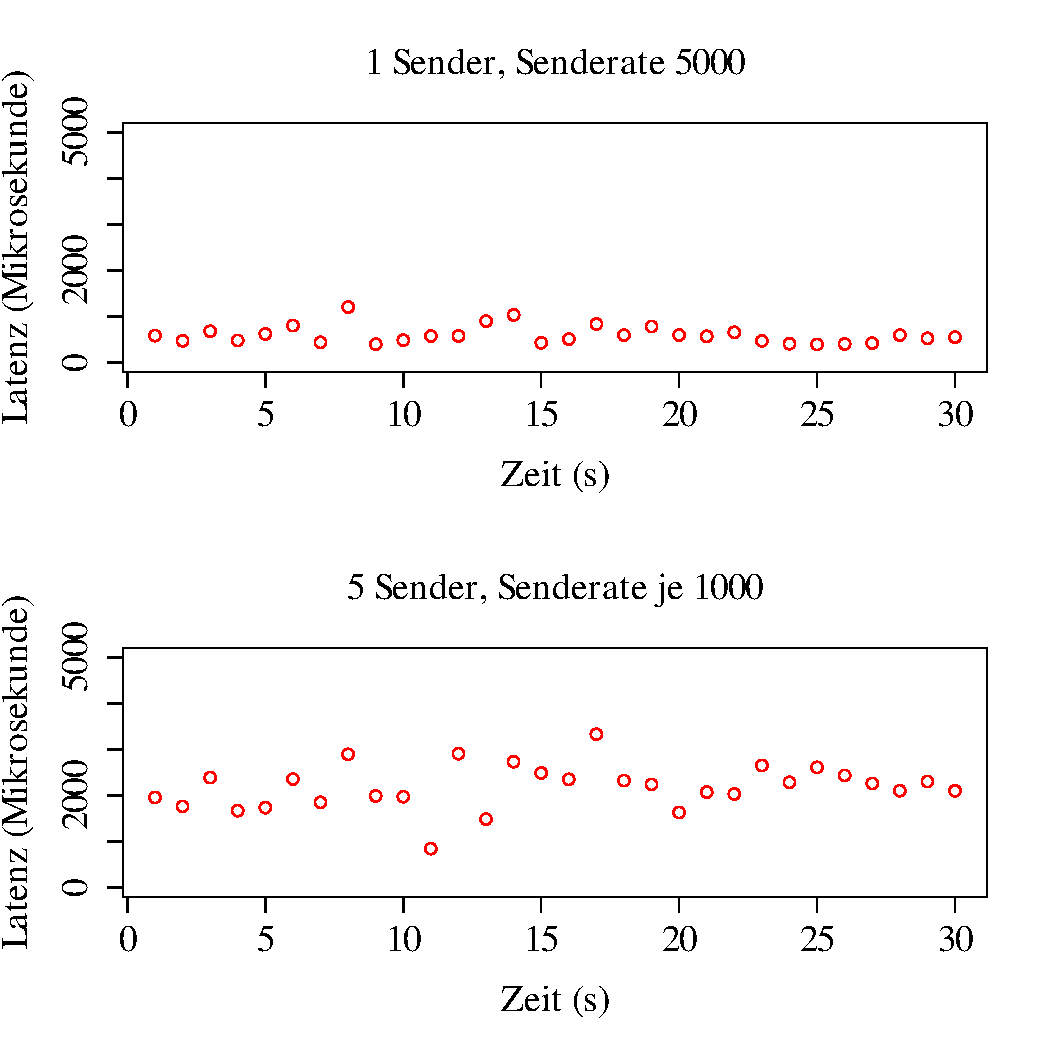
\includegraphics[width=1\textwidth]{images/measurement/varying-producer.pdf}
  \caption{Verschiedene Sender Anzahl}
  \label{img:varyingProducer}
\end{figure}
%E
Diese Messung zeigt, dass er vernachlaessigbar ist ob ein Sender oder mehrere Sender benutzt werden um eine bestimmte Senderate zu erreichen. 
%A
%In einer weiteren Messung sollte Ausserdem geprueft werden, ob mehrere Sender ohne Sendelimit mehr Nachrichten senden koennen als ein Sender. Dazu wurde der selbe Versuchsaufbau wie oben gewaehlt mit dem Unterschied, dass diesmal die Senderate nicht eingeschraenk wurde.
%B
%In \autoref{img:varyingProducerMaxThroughput} sind die Ergebnisse dargestellt. Dabei ist zu sehen, dass die 5 Sender zusammen genauso viele Nachrichten senden wie ein Sender allein. Ausserdem ist die Latenz im Fall der 5 Sender um ein 5faches groesser als bei einem Sender.
%\begin{figure}
%\center
%  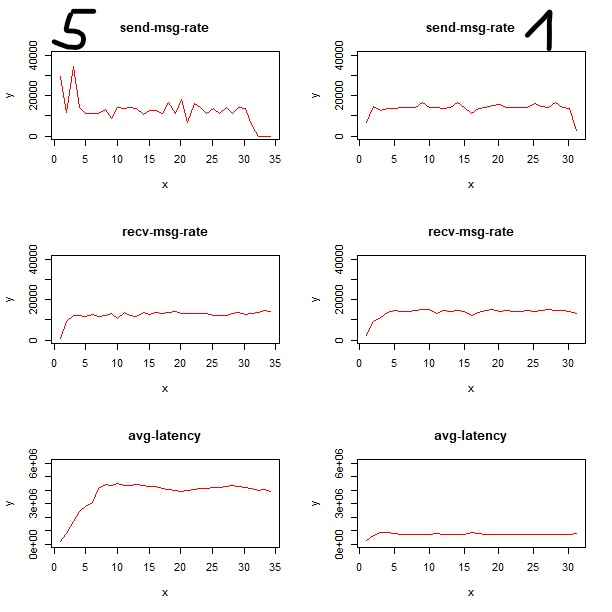
\includegraphics[width=1\textwidth]{images/varyingProducerMaxThroughput.jpg}
%  \caption{Verschiedene Sender Anzahl}
%  \label{img:varyingProducerMaxThroughput}
%\end{figure}
%E
%Das die 5 Sender jeweils nur 1/5 der moeglichen Senderate senden, kann dadurch erklaert werden, dass das Testsystem nicht mehr als eine bestimmte Rate an Nachrichten senden kann. D.h. das es keinen Unterschied macht ob ein Sender oder mehrere Sender Nachrichten senden. DIeses Verhalten kann sich aendern, wenn sich verschiedene Sender auf verschiedenen Maschinen befinden. (evtl noch Messung durchfuehren um zu zeigen) 


%Ableitung von ResourceDemands -> Regressionsfkt

%\subsection{ActiveMQ}
%ActiveMQ \cite{activeMQ} ist eine Open-Source-MOM, die seit 2004 kontinuierlich weiter entwickelt wird. ActiveMQ ist in Java geschrieben und implementiert den Java Message Service (JMS) \cite{jms}. Dabei handelt es sich um eine Programmierschnittstelle zur Ansteuerung einer MOM. Dabei soll eine lose gekoppelte, verlässliche und asynchrone Kommunikation zwischen den Komponenten einer verteilten Anwendung ermöglicht werden. ActiveMQ verfügt außerdem über mehrere Betriebsarten für hohe Verfügbarkeit und einen robusten horizontalen Skalierungsmechanismus. Darüber hinaus ist es sehr flexibel in der Konfiguration und unterstützt eine Vielzahl von Transportprotokollen, darunter auch AMQP.

\subsection{Zusammenfassung}
welche Einflussfaktoren konnnten identifiziert werden und werden weiter betrachtet? \\
Nachrichtengroesse hat einfluss auf Latenz, Senderate und gesendete Datenmenge \\
%Througput der Verbindung (linking Ressource)\\
%Msg rate des Senders und Empfaengers (ankunftsrate im Usage modell) \\
%Nachrichtengroesse und ihre Latenz (response time einer Nachricht) \\
Netzwerklatenz \\
Moegliche Datenmenge ist durch Netzwerk begrenzt\\
Ob Nachrichten in HS oder HDD gespeichert werden (lazy queues) \\
Kein Unterschied ob ein oder mehrere Sender/Empfaenger Warteschlange fuellen/abarbeiten \\

welche weiteren Einflussfaktoren gibt es, die aus bestimmten gruenden nicht betrachtet werden (koennen)\\
wenn system mehr Nachrichten auf einmal sendet/empfaengt sinkt latenz wieder \\
RMQ hat auch Prefetch von Nachrichten. Wird nicht betrachtet (zeit und trotzdem nicht so gut wie kafka) \\
Latenz steigt an, wenn die queue gefuellt wird \\
- benoetigt tracken einer Nachricht durch das system \\
- explizite Queue Modellierung, mit groesse und fuellstand \\


%--	Vergleich: https://stackshare.io/stackups/activemq-vs-kafka-vs-rabbitmq  \\


